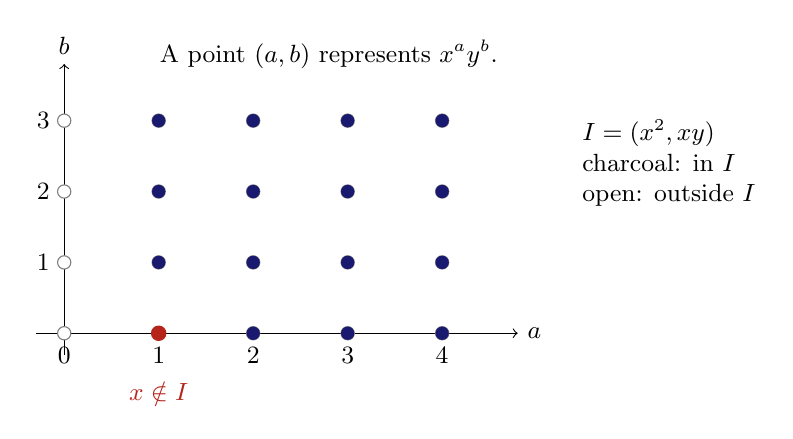
\begin{tikzpicture}[font=\small,x=1.2cm,y=0.9cm]
\draw[->] (-0.3,0)--(4.8,0) node[right] {$a$};
\draw[->] (0,-0.3)--(0,3.8) node[above] {$b$};
\foreach \a in {0,...,4} {\node[below] at (\a,-0.06) {$\a$};}
\foreach \b in {1,...,3} {\node[left] at (-0.05,\b) {$\b$};}
\foreach \a in {0,...,4} {\foreach \b in {0,...,3} {
  \fill[white] (\a,\b) circle (2.4pt);
  \draw[gray] (\a,\b) circle (2.4pt);
}}
\foreach \a in {2,...,4} {\foreach \b in {0,...,3} {
  \fill[MidnightBlue] (\a,\b) circle (2.4pt);
}}
\foreach \b in {1,...,3} {\fill[MidnightBlue] (1,\b) circle (2.4pt);}
\fill[BrickRed] (1,0) circle (2.8pt);
\node[BrickRed,below] at (1,-0.55) {$x\notin I$};
\node[above,align=center] at (2.8,3.6) {A point $(a,b)$ represents $x^ay^b$.};
\node[align=left] at (6.4,2.4) {$I=(x^2,xy)$\\charcoal: in $I$\\open: outside $I$};
\end{tikzpicture}
